\documentclass[tikz,border=10pt]{standalone}
\usetikzlibrary{arrows.meta,positioning}

\begin{document}
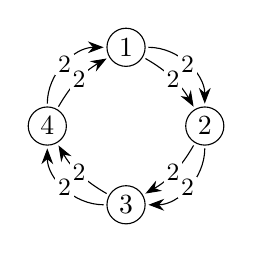
\begin{tikzpicture}[
    vertex/.style={circle, draw=black, fill=white, inner sep=2pt},
    edge_label/.style={font=\small, midway, fill=white, inner sep=1pt},
    arrow/.style={-{Stealth[length=2mm]}, shorten >=1pt, shorten <=1pt}
]
    % Vertices
    \node[vertex] (v1) at (0,1) {1};
    \node[vertex] (v2) at (1,0) {2};
    \node[vertex] (v3) at (0,-1) {3};
    \node[vertex] (v4) at (-1,0) {4};

    % Edges and labels (clockwise)
    \draw[arrow] (v1) to[bend left=15] node[edge_label] {2} (v2);
    \draw[arrow] (v1) to[bend left=45] node[edge_label] {2} (v2);
    \draw[arrow] (v2) to[bend left=15] node[edge_label] {2} (v3);
    \draw[arrow] (v2) to[bend left=45] node[edge_label] {2} (v3);
    \draw[arrow] (v3) to[bend left=15] node[edge_label] {2} (v4);
    \draw[arrow] (v3) to[bend left=45] node[edge_label] {2} (v4);
    \draw[arrow] (v4) to[bend left=15] node[edge_label] {2} (v1);
    \draw[arrow] (v4) to[bend left=45] node[edge_label] {2} (v1);

    % Counterclockwise edges (optional, if bidirectional)
    % Uncomment if counterclockwise edges are required:
    % \draw[arrow, dashed] (v2) to[bend right=15] node[edge_label] {2} (v1);
    % \draw[arrow, dashed] (v3) to[bend right=15] node[edge_label] {2} (v2);
    % \draw[arrow, dashed] (v4) to[bend right=15] node[edge_label] {2} (v3);
    % \draw[arrow, dashed] (v1) to[bend right=15] node[edge_label] {2} (v4);
\end{tikzpicture}
\end{document}